\begin{figure}[htbp]
    \centering
    
\includegraphics[width=0.92\textwidth]{figures/fig00_geometry_material_model.png}
    \caption{Single-element Abaqus validation model and Chaboche-v1 material-state workflow. The block is a one-element C3D8 specimen with \(L_0=10~\mathrm{mm}\), a \(2~\mathrm{mm}\times2~\mathrm{mm}\) cross-section, fixed left face, and displacement-controlled cyclic loading on the right face.}
    \label{fig:geometry_material_model}
\end{figure}

\begin{figure}[htbp]
    \centering
    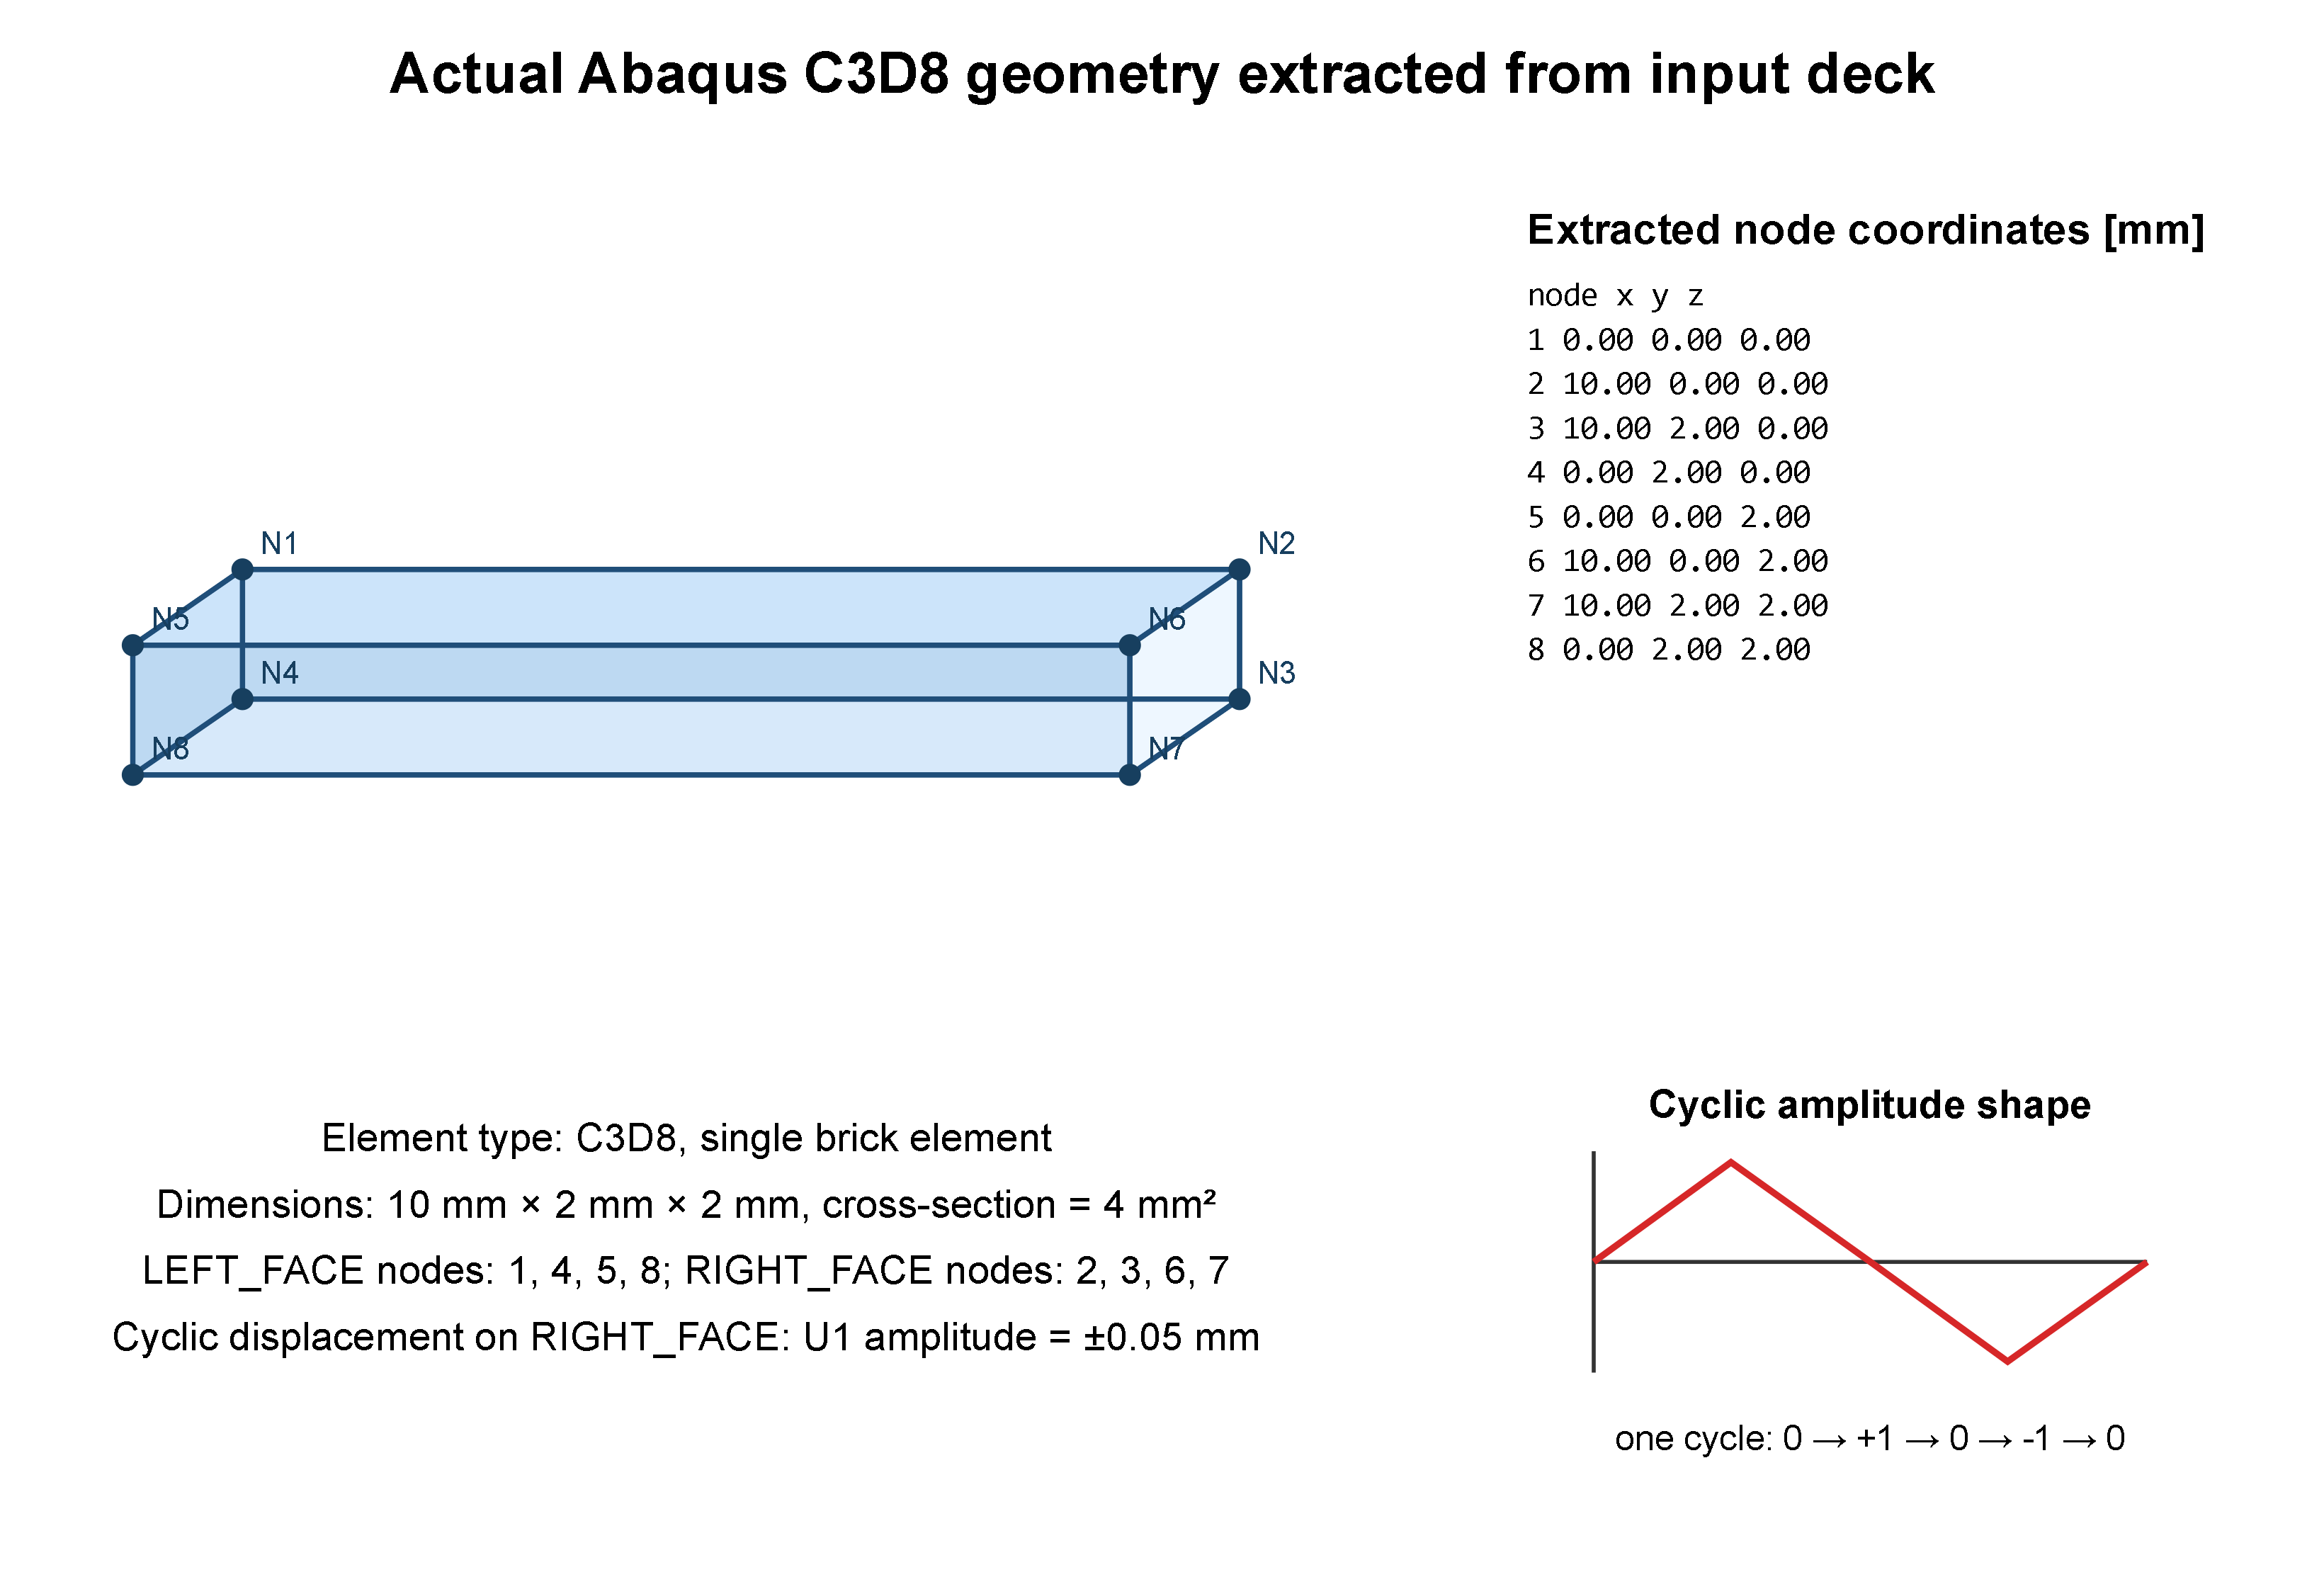
\includegraphics[width=0.92\textwidth]{figures/fig00b_actual_abaqus_geometry.png}
    \caption{Actual Abaqus single-element geometry reconstructed from the input deck using the node coordinates and C3D8 element connectivity. The extracted model confirms the \(10~\mathrm{mm}\times2~\mathrm{mm}\times2~\mathrm{mm}\) block, the left and right node sets, and the displacement-controlled cyclic loading direction.}
    \label{fig:actual_abaqus_geometry}
\end{figure}

\begin{figure}[htbp]
    \centering
    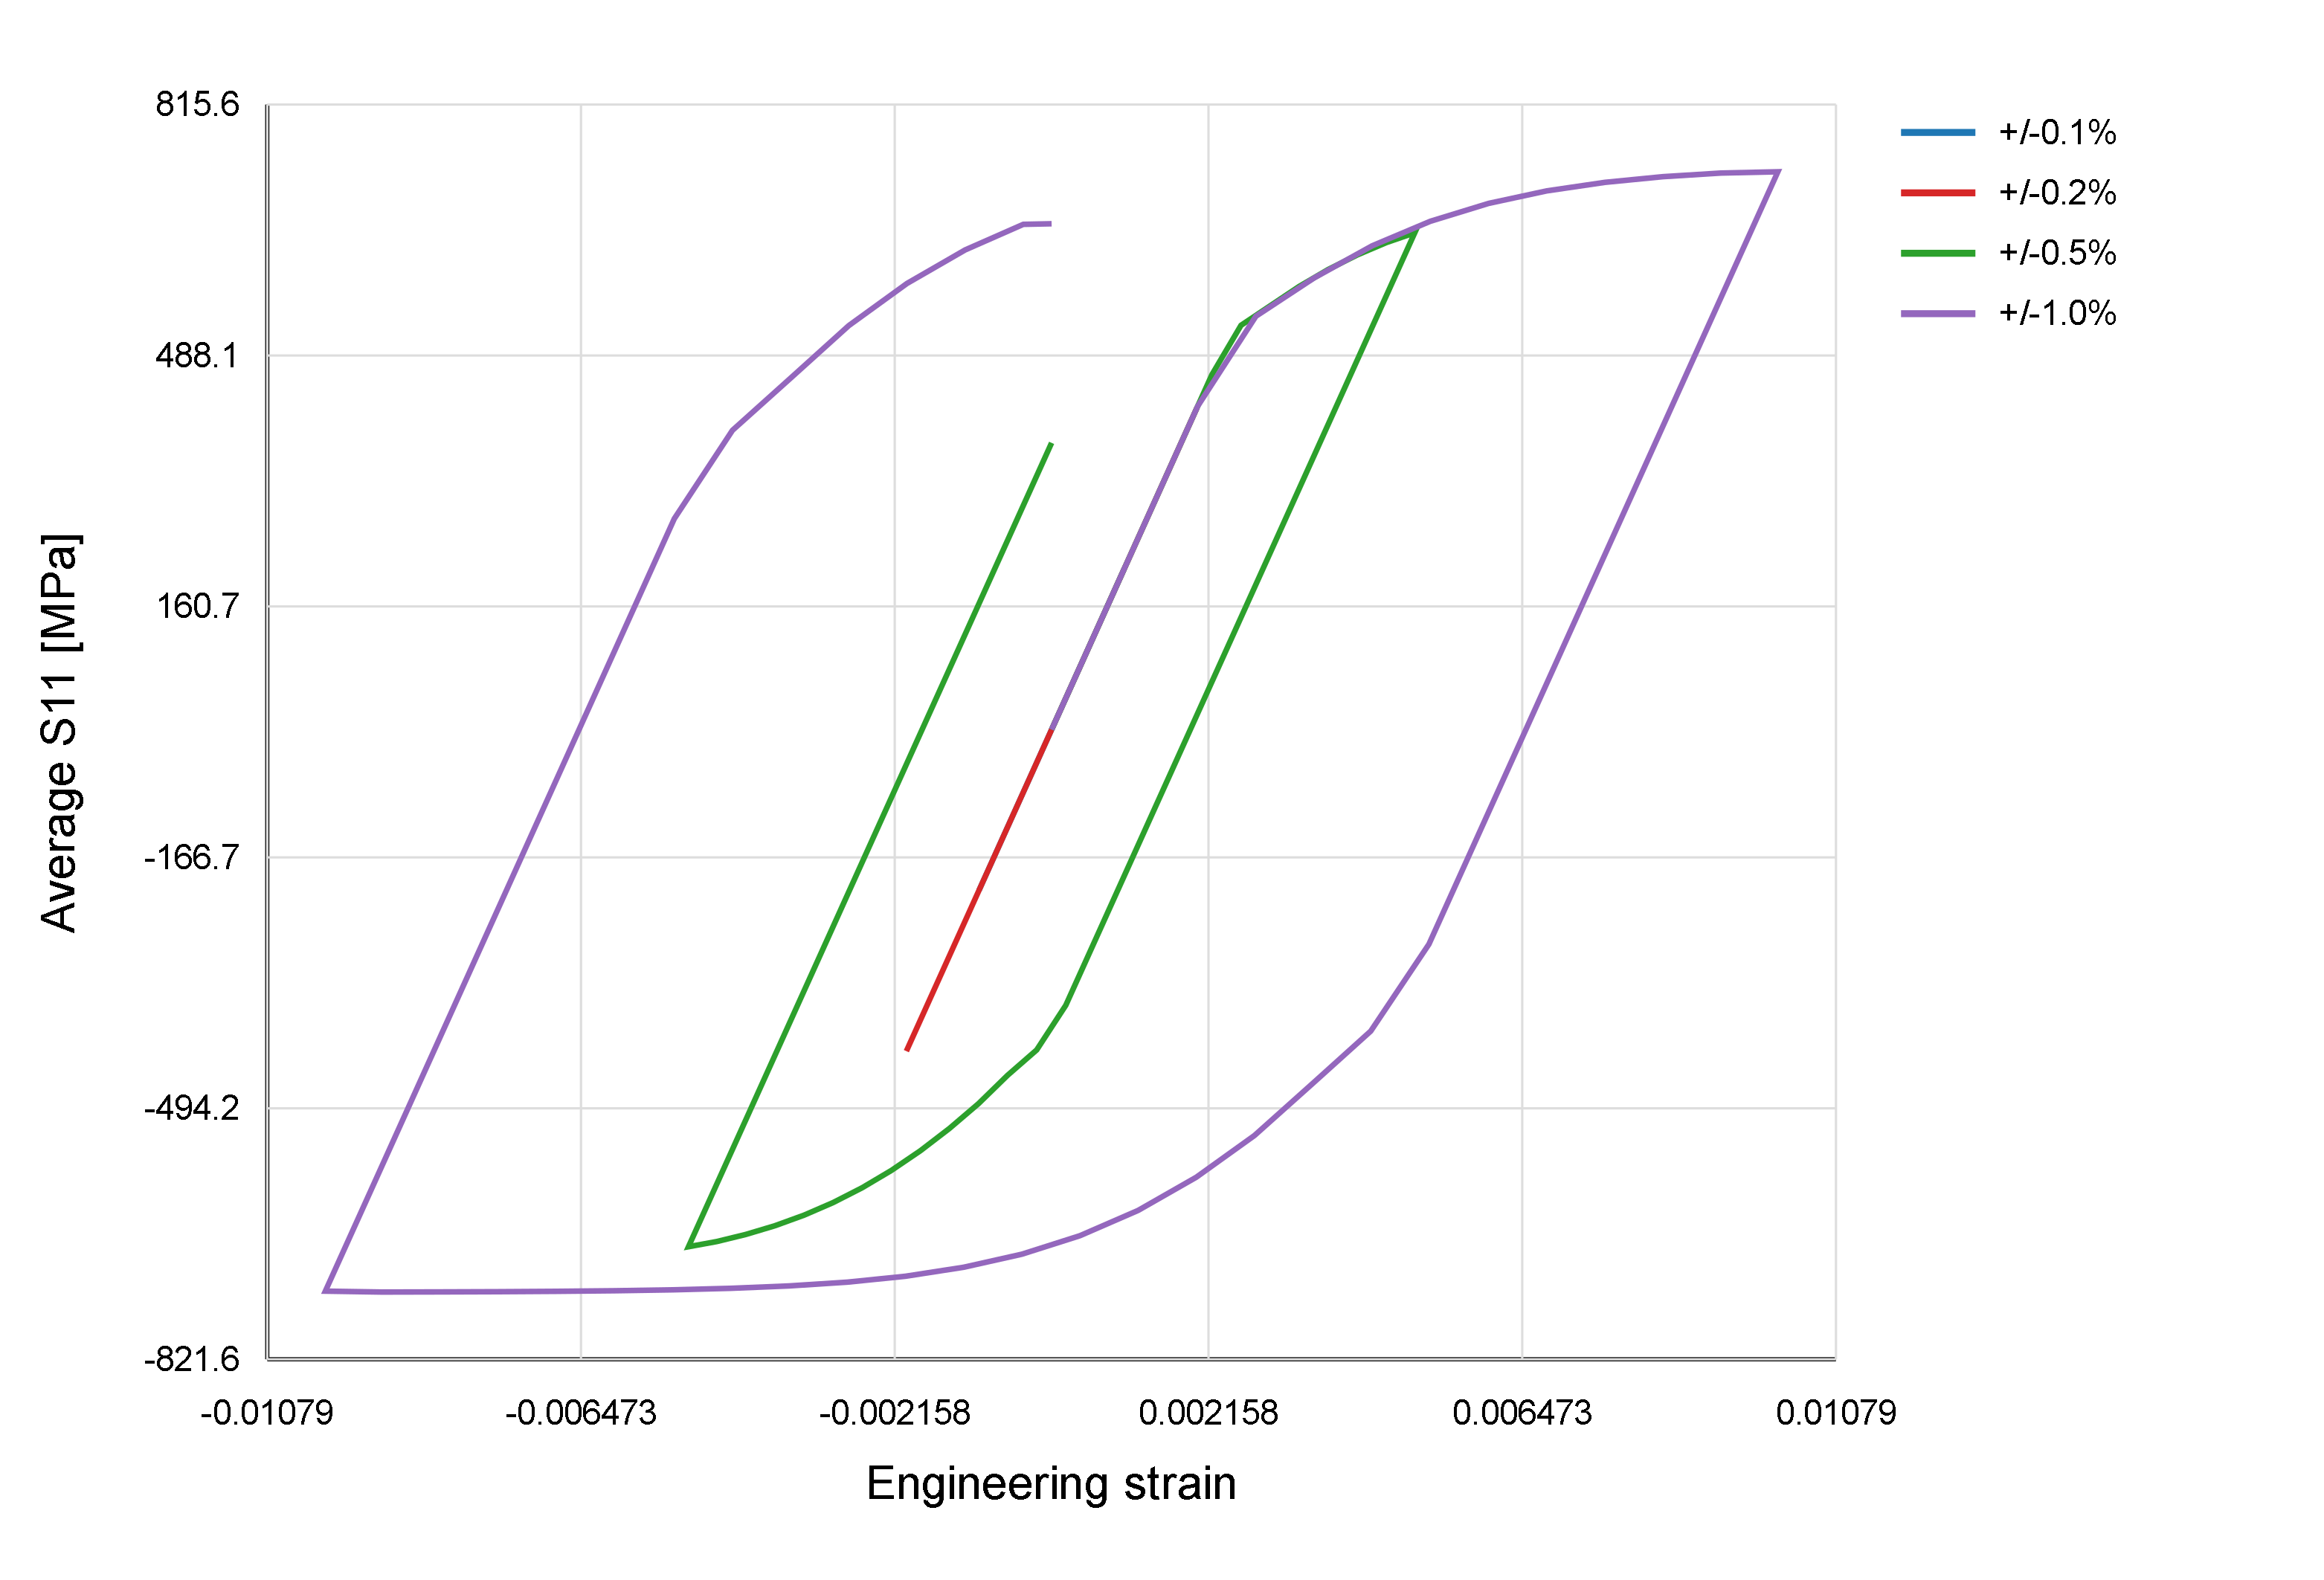
\includegraphics[width=0.82\textwidth]{figures/fig01_amplitude_sweep_stress_strain.png}
    \caption{Amplitude sweep for the Chaboche-v1 UMAT. The smaller amplitudes remain mainly elastic, while the $\pm0.5\%$ case activates viscoplasticity at a moderate stress level and was selected for the cycle-jump demonstration.}
    \label{fig:amplitude_sweep}
\end{figure}

\begin{figure}[htbp]
    \centering
    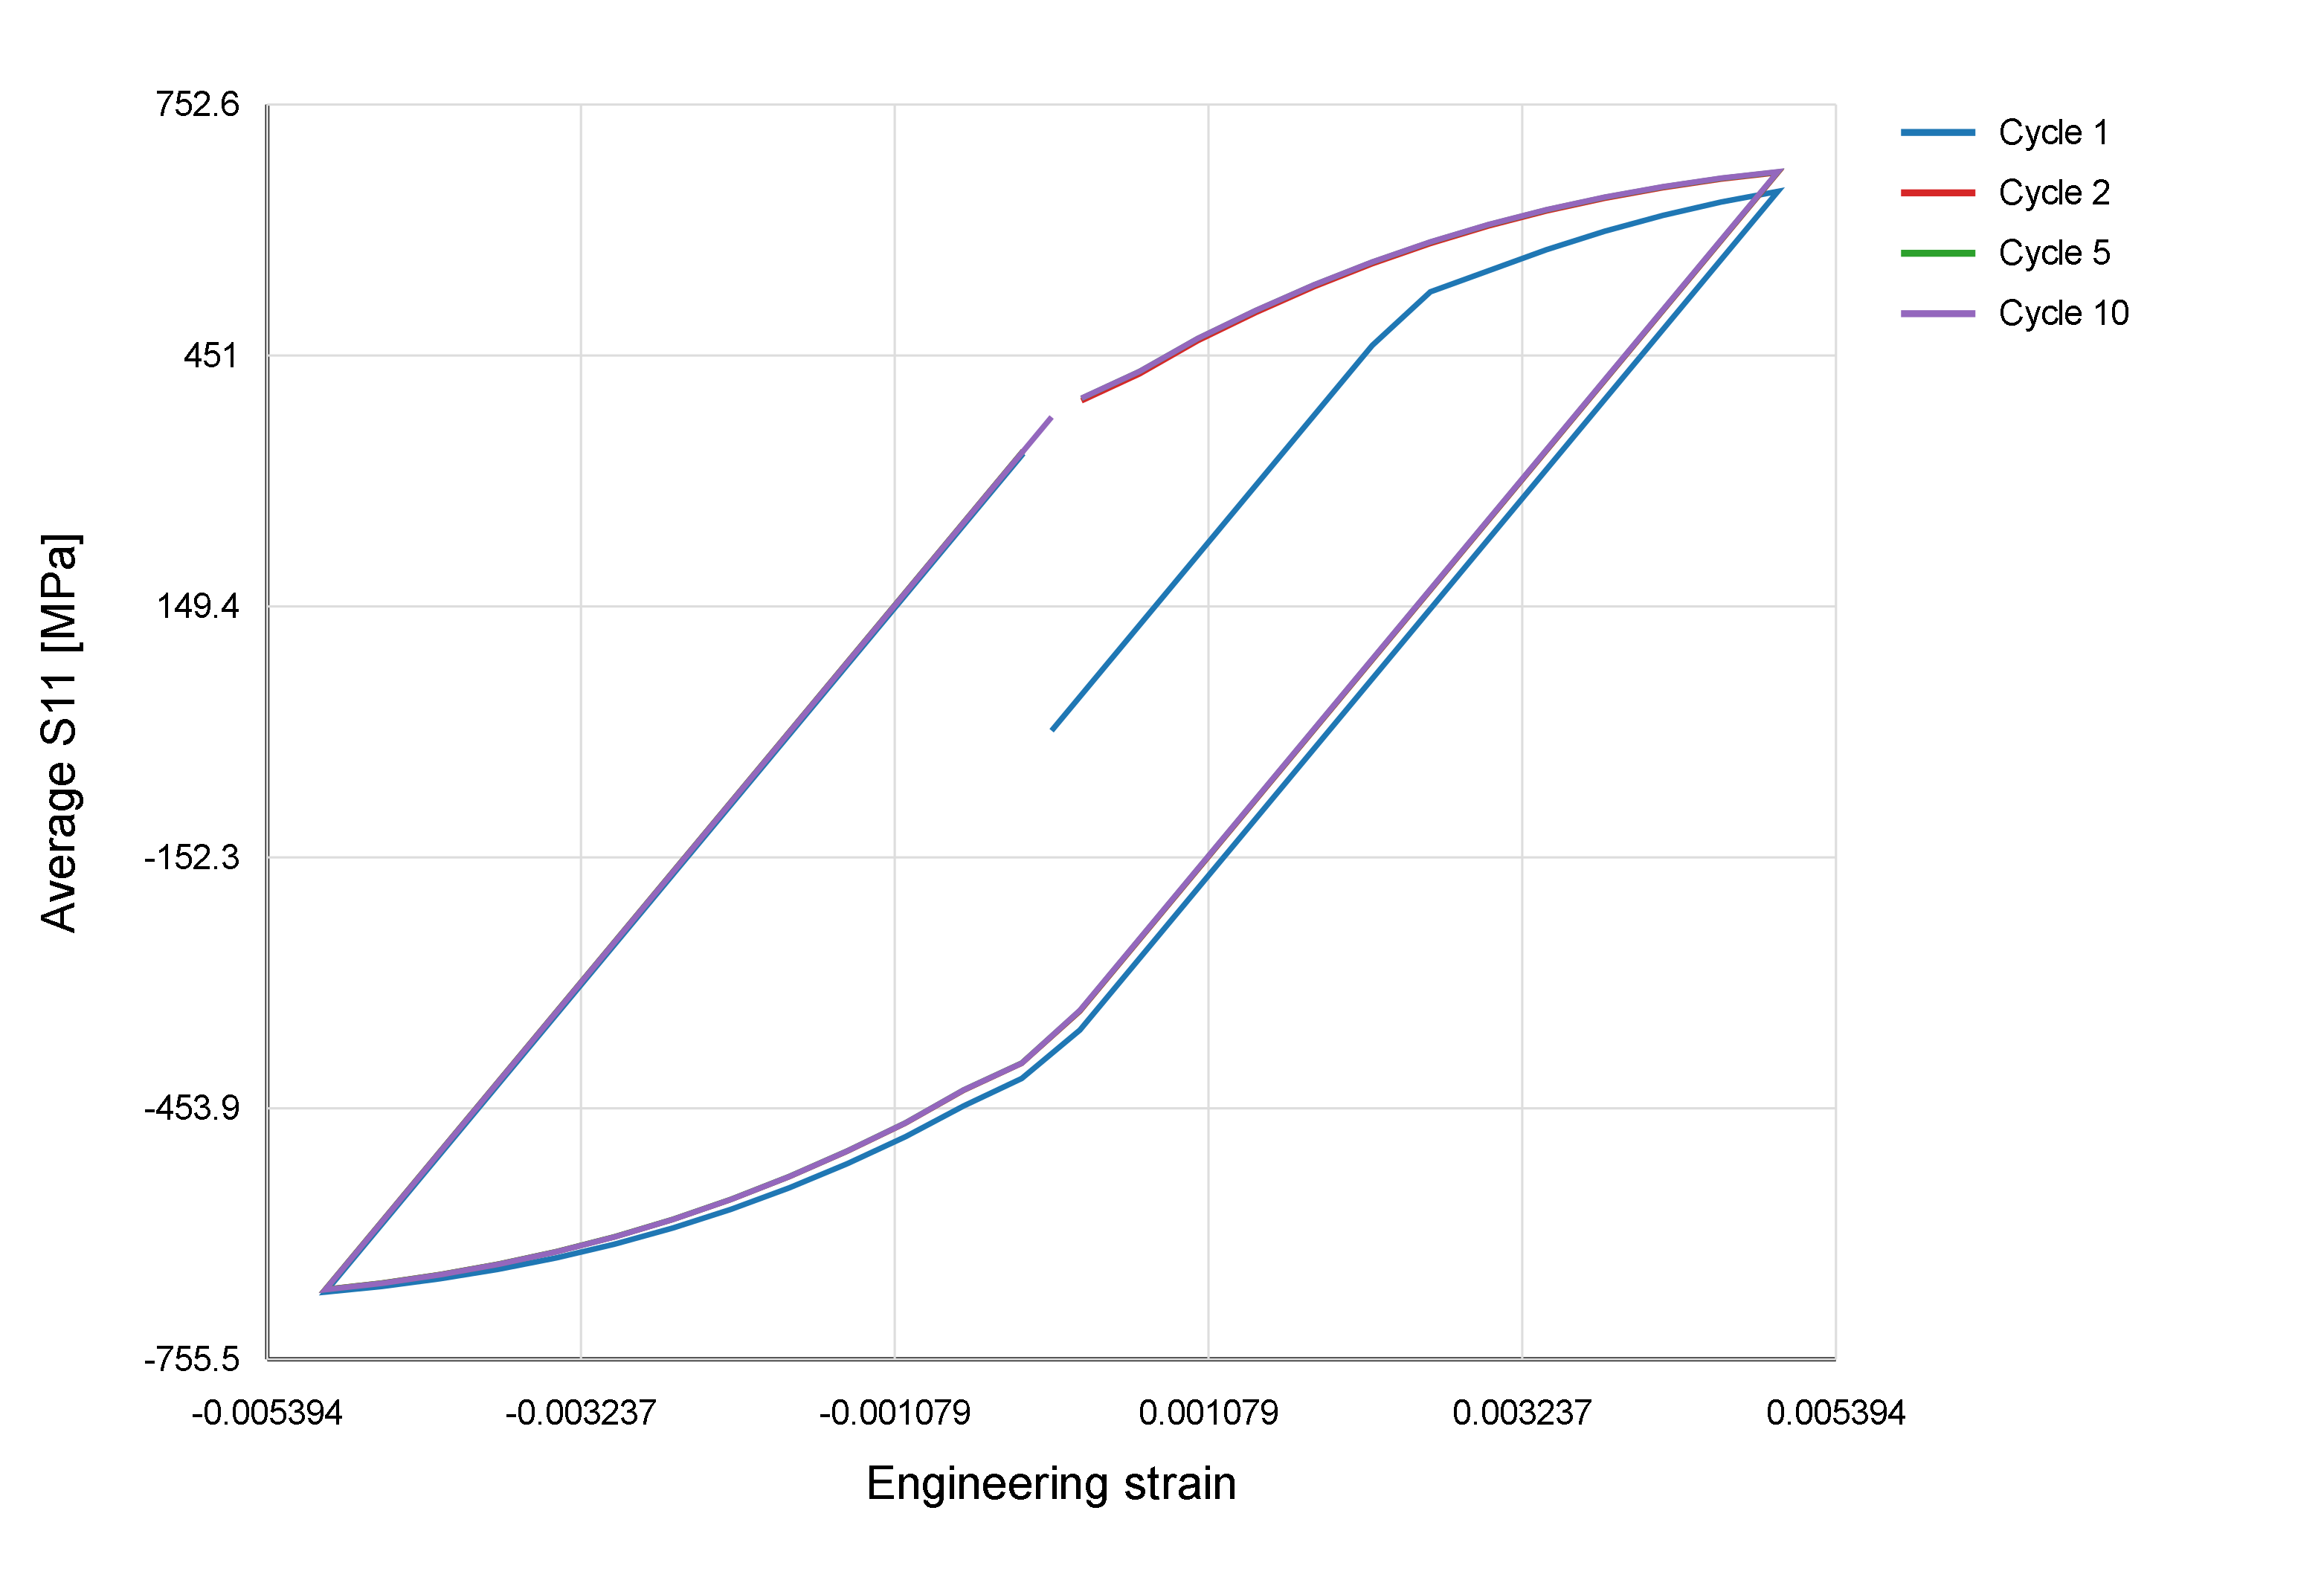
\includegraphics[width=0.82\textwidth]{figures/fig02_10cycle_selected_hysteresis_loops.png}
    \caption{Selected hysteresis loops from the explicit 10-cycle Abaqus simulation at $\pm0.5\%$ strain amplitude. The loop shape becomes nearly repeatable after the initial transient.}
    \label{fig:ten_cycle_loops}
\end{figure}

\begin{figure}[htbp]
    \centering
    
\includegraphics[width=0.82\textwidth]{figures/fig03_delta_sdv1_per_cycle.png}
    \caption{Per-cycle increment of accumulated viscoplastic strain. After the first cycle, the increment remains nearly constant, supporting the use of a cycle-jump predictor.}
    \label{fig:delta_sdv1}
\end{figure}

\begin{figure}[htbp]
    \centering
    
\includegraphics[width=0.82\textwidth]{figures/fig04_cycle_jump_sdv1_prediction.png}
    \caption{Cycle-jump prediction of accumulated viscoplastic strain using the stabilized per-cycle increment obtained from explicit cycles 2--10.}
    \label{fig:jump_prediction}
\end{figure}

\begin{figure}[htbp]
    \centering
    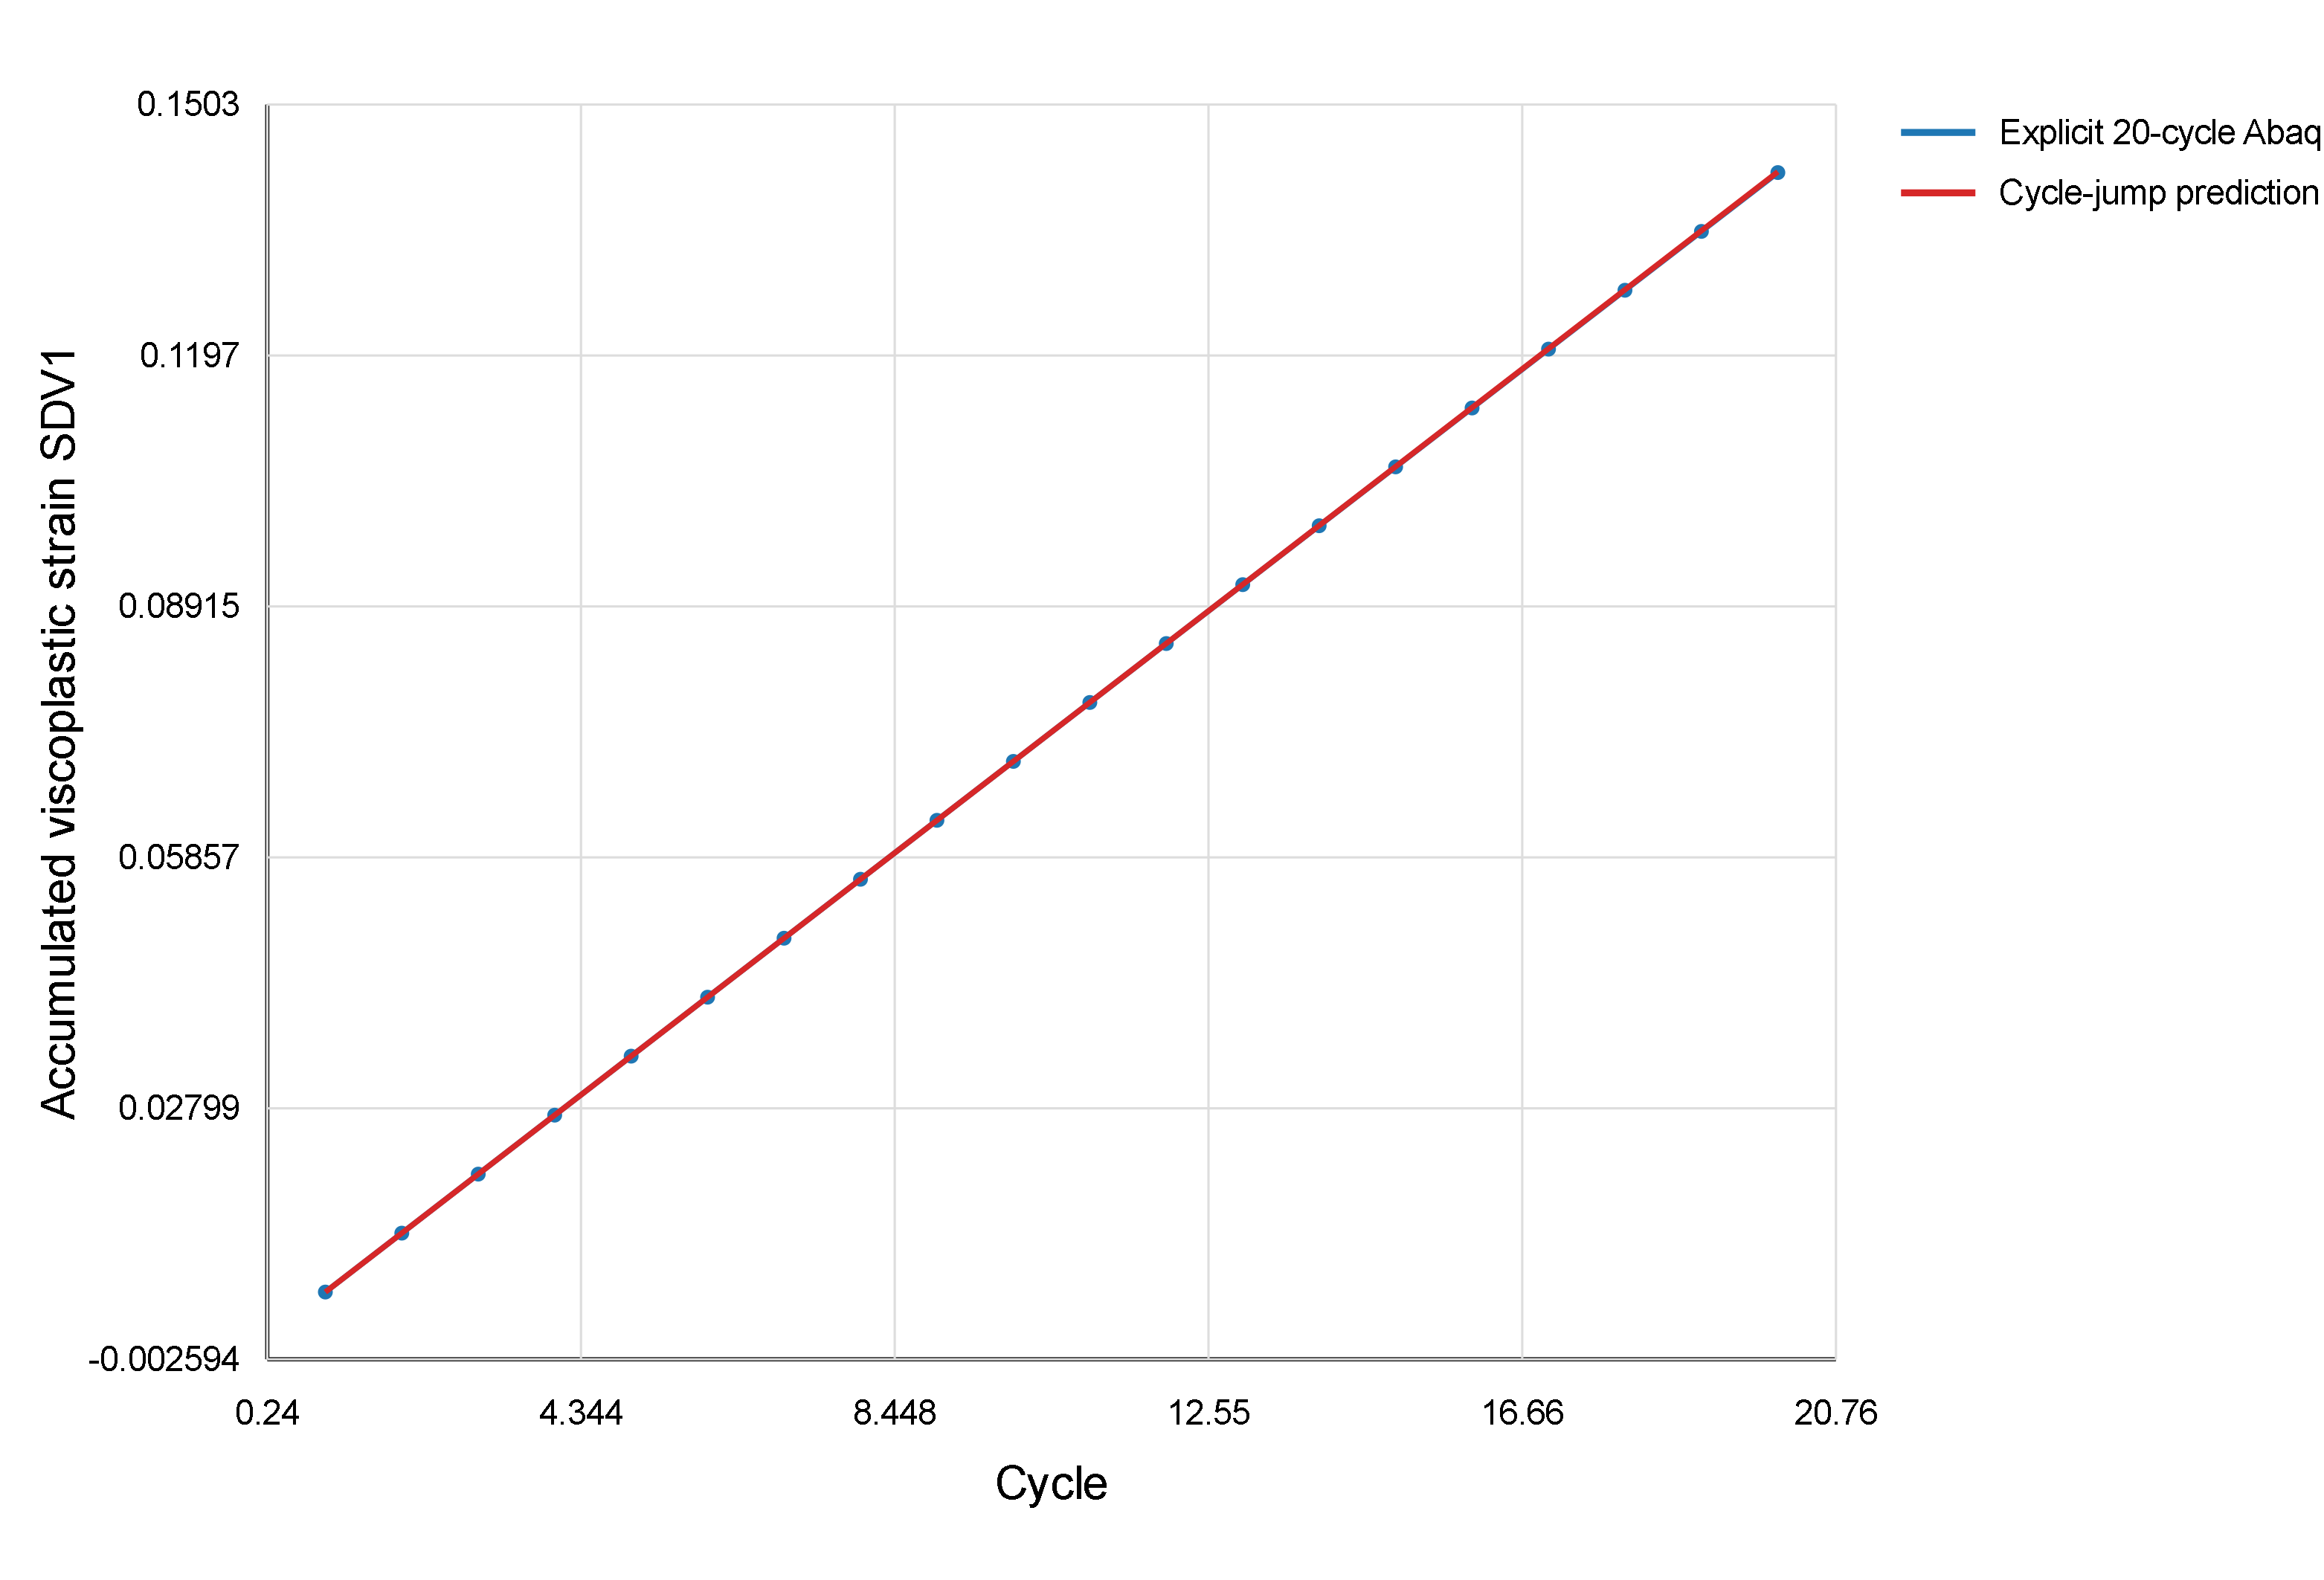
\includegraphics[width=0.82\textwidth]{figures/fig05_cycle_jump_vs_explicit_20cycles.png}
    \caption{Validation of the cycle-jump predictor against an independent explicit 20-cycle Abaqus simulation. The predicted and explicit SDV1 values agree closely, with a relative error of 0.0674\% at cycle 20.}
    \label{fig:jump_validation}
\end{figure}
